% Baccalauréat malgache, série C, 2015 : corrigé.
\TCDBacAttribution{C}{2015}
\providecommand{\cm}{~\mathrm{cm}}
\providecommand{\dx}{~\mathrm{d}x}
\providecommand{\bary}[1]{\mathrm{bar}\left\lbrace #1 \right\rbrace}
\providecommand{\Angl}[2]{\left( \widehat{ \overrightarrow{#1} , \overrightarrow{#2} } \right)}
%
%%%%%%%%%%%%%%%%%%%%%%%%%%%%%%%%%%%%%%%%%%%%%%%%%%%%%%%%%%%%%%%%%%%%%%%%%%%%%%%%%%%%%%%%%%%%%%%%%%%%%%%%%%%%%%%%%%%%%%%%%%%%%%%%
\noindent \underline{\textsc{\textbf{Exercice}}} (4 points)
\begin{description}
	\item[I.]
	\begin{enumerate}
		\item \vln{Équation dans $\mathbb{Z}/7\mathbb{Z}$ :}
			$-\bar{3} = \bar{4}$, donc $\bar{6}x = \bar{4} - \bar{2} = \bar{2}$. Or $\bar{6} = -\bar{1}$, d'où $x = -\bar{2} = \bar{5}$.
			Vérification : $\bar{6} \times \bar{5} + \bar{2} = \bar{32} = \bar{4} = -\bar{3}$.
			\par\noindent\ansbox{$S = \{\bar{5}\}$.}
		\item \vln{$A$ et $B$ premiers entre eux :}
			$5A - 3B = 25a + 15b - 24a - 15b = a$ et $5B - 8A = 40a + 25b - 40a - 24b = b$.
			Un diviseur commun $d$ de $A$ et $B$ divise donc $a$ et $b$, donc divise $\pgcd{a}{b} = 1$.
			\par\noindent\ansbox{$\pgcd{A}{B} = 1$ : $A$ et $B$ sont premiers entre eux.}
		\item $M = 2 \times 13^3 + 5 \times 13^2 + x \times 13 + 3$, où $x$ est un chiffre de la base $13$ : $0 \leq x \leq 12$.
		\begin{enumerate}
			\item \vln{Congruence modulo $4$ :}
				$13 = 3 \times 4 + 1 \equiv 1 \pmod 4$, donc $13^k \equiv 1$ et $M \equiv 2 + 5 + x + 3 = x + 10 \equiv x + 2 \pmod 4$.
				\par\noindent\ansbox{$M \equiv x + 2 \ [4]$.}
			\item \vln{Divisibilité par $4$ :}
				$4 \mid M \iff x + 2 \equiv 0 \iff x \equiv 2 \pmod 4$. Avec $0 \leq x \leq 12$ :
				\par\noindent\ansbox{$x \in \{2 \, ; 6 \, ; 10\}$.}
		\end{enumerate}
	\end{enumerate}
	\item[II.]
	\begin{enumerate}
		\item Le dé est parfait : chacune des quatre faces est cachée avec la probabilité $\frac{1}{4}$.
		\begin{description}
			\item[A :] \vln{Face cachée $\leq 4$ :}
				faces $2$, $3$, $4$ : \par\noindent\ansbox{$P(A) = \frac{3}{4}$.}
			\item[B :] \vln{Somme des faces visibles première :}
				$2 + 3 + 4 + 5 = 14$ ; la somme visible est $14 - h$ où $h$ est le numéro caché : $12$, $11$, $10$, $9$ pour $h = 2, 3, 4, 5$.
				Seul $11$ est premier. \par\noindent\ansbox{$P(B) = \frac{1}{4}$.}
		\end{description}
		\item Les lancers sont indépendants ; l'événement contraire de « au moins une fois $A$ » est « jamais $A$ », de probabilité $\left(\frac{1}{4}\right)^n$.
			Donc $P_n = 1 - \left(\frac{1}{4}\right)^n$.
		\begin{enumerate}
			\item \vln{Calcul de $P_3$ :}
				\ansbox{$P_3 = 1 - \frac{1}{64} = \frac{63}{64}$.}
			\item \vln{Plus petit $n$ :}
				$P_n \geq 0{,}99 \iff \left(\frac{1}{4}\right)^n \leq \frac{1}{100} \iff 4^n \geq 100$. Or $4^3 = 64 < 100 \leq 256 = 4^4$.
				\par\noindent\ansbox{$n = 4$.}
		\end{enumerate}
	\end{enumerate}
\end{description}
%%%%%%%%%%%%%%%%%%%%%%%%%%%%%%%%%%%%%%%%%%%%%%%%%%%%%%%%%%%%%%%%%%%%%%%%%%%%%%%%%%%%%%%%%%%%%%%%%%%%%%%%%%%%%%%%%%%%%%%%%%%%%%%%
\noindent \underline{\textsc{\textbf{PROBLEME I}}} (7 points) \newline
Rappels sur l'hexagone régulier de côté $a$ : les triangles $OAB$, $OBC$, \ldots{} sont équilatéraux de côté $a$ ;
deux sommets séparés d'un sommet sont à la distance $a\sqrt{3}$ (petite diagonale) ; deux sommets opposés sont à la distance $2a$.
\begin{center}
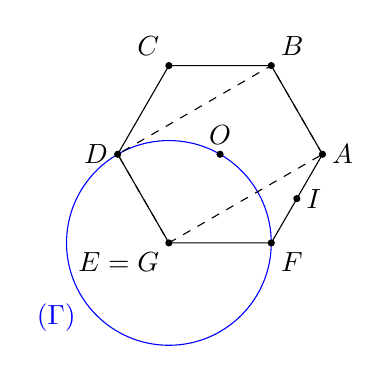
\begin{tikzpicture}[scale=1.3]
	\foreach \k/\N in {0/A,1/B,2/C,3/D,4/E,5/F} \coordinate (\N) at ({60*\k}:1);
	\coordinate (O) at (0,0); \coordinate (I) at (0.75,-0.433);
	\draw (A) -- (B) -- (C) -- (D) -- (E) -- (F) -- cycle;
	\draw[blue] (E) circle (1);
	\draw[dashed] (A) -- (B) -- (D) -- (E) -- cycle;
	\foreach \P/\pos in {A/right,B/above right,C/above left,D/left,F/below right,O/above,I/right}
		\fill (\P) circle (1pt) node[\pos] {$\P$};
	\fill (E) circle (1pt) node[below left] {$E = G$};
	\node[blue] at (-1.6,-1.6) {$(\Gamma)$};
\end{tikzpicture}
\end{center}
\begin{description}
	\item[Partie A]
	\begin{enumerate}
		\item \vln{Barycentre $G$ :}
			La somme des poids vaut $1$ ; $\overrightarrow{AG} = -\overrightarrow{AB} + \overrightarrow{AD} = \overrightarrow{BD}$.
			Le quadrilatère $ABDE$ est un rectangle (ses diagonales $[AD]$ et $[BE]$ sont deux diamètres du cercle circonscrit), donc $\overrightarrow{BD} = \overrightarrow{AE}$.
			\par\noindent\ansbox{$G = E$.}
		\item
		\begin{enumerate}
			\item \vln{Ensemble $(\Gamma)$ :}
				Relation de Leibniz (somme des poids $1$) : $MA^2 - MB^2 + MD^2 = MG^2 + GA^2 - GB^2 + GD^2$.
				Avec $G = E$ : $EA^2 = 3a^2$, $EB^2 = 4a^2$, $ED^2 = a^2$ ; la constante est nulle.
				La condition devient $ME^2 = a^2$.
				\par\noindent\ansbox{$(\Gamma)$ est le cercle de centre $E$ et de rayon $a$.}
			\item \vln{Passage par $O$ :}
				$EO = a$ (triangle $OED$ équilatéral), donc \par\noindent\ansbox{$O \in (\Gamma)$.} ($(\Gamma)$ passe aussi par $D$ et $F$.)
		\end{enumerate}
	\end{enumerate}
	\item[Partie B]
	\textbf{1\textsuperscript{re} méthode.}
	\begin{enumerate}
		\item \vln{$f$ est une symétrie centrale :}
			$f$ est la composée de deux rotations d'angles $\frac{\pi}{3}$ et $\frac{2\pi}{3}$ : c'est un déplacement d'angle $\pi$, donc une rotation d'angle $\pi$.
			\par\noindent\ansbox{$f$ est une symétrie centrale.}
		\item \vln{Image de $A$ et centre :}
			$R_O(A) = B$ ($OA = OB$, $\Angl{OA}{OB} = \frac{\pi}{3}$, hexagone direct). $R_A(B) = F$ car $AB = AF$ et $\Angl{AB}{AF} = \frac{2\pi}{3}$.
			Donc $f(A) = F$ ; le centre d'une symétrie centrale est le milieu d'un point et de son image.
			\par\noindent\ansbox{$f(A) = F$ et $f$ est la symétrie de centre $I$, milieu de $[AF]$.}
	\end{enumerate}
	\textbf{2\textsuperscript{e} méthode.} (L'unité est $OA = a$.)
	\begin{enumerate}
		\item \vln{Affixes :}
			$z_A = 1$ ; $F$ est l'image de $A$ par la rotation de centre $O$ et d'angle $-\frac{\pi}{3}$ : $z_F = \expo{-i\frac{\pi}{3}}$.
			\par\noindent\ansbox{$z_A = 1$, $z_F = \frac{1}{2} - \frac{\sqrt{3}}{2}i$, $z_I = \frac{3}{4} - \frac{\sqrt{3}}{4}i$.}
		\item \vln{Expressions complexes :}
			\par\noindent\ansbox{$R_O : z' = \expo{i\frac{\pi}{3}}z$ ; $R_A : z' = \expo{i\frac{2\pi}{3}}(z - 1) + 1$.}
			$f(z) = \expo{i\frac{2\pi}{3}}\left(\expo{i\frac{\pi}{3}}z - 1\right) + 1 = \expo{i\pi}z - \expo{i\frac{2\pi}{3}} + 1 = -z + 1 + \frac{1}{2} - \frac{\sqrt{3}}{2}i$.
			\par\noindent\ansbox{$f : z' = -z + \frac{3}{2} - \frac{\sqrt{3}}{2}i$.}
		\item \vln{Nature :}
			$z' = -z + b$ : symétrie centrale de centre d'affixe $\frac{b}{2} = \frac{3}{4} - \frac{\sqrt{3}}{4}i = z_I$.
			\par\noindent\ansbox{$f$ est la symétrie centrale de centre $I$.}
	\end{enumerate}
	\item[Partie C]
	\begin{enumerate}
		\item
		\begin{enumerate}
			\item \vln{$g(A)$ :}
				$g$ est la rotation de centre $O$ et d'angle $\frac{2\pi}{3}$ ; $g(A) = R_O(B) = C$. \par\noindent\ansbox{$g(A) = C$.}
			\item \vln{Écriture complexe :}
				\ansbox{$g : z' = \expo{i\frac{2\pi}{3}}z = \left(-\frac{1}{2} + \frac{\sqrt{3}}{2}i\right)z$.}
			\item \vln{Affixes de $C$ et $E$ :}
				$z_C = g(1)$ et $E = g(C)$ :
				\par\noindent\ansbox{$z_C = -\frac{1}{2} + \frac{\sqrt{3}}{2}i$ et $z_E = \expo{i\frac{4\pi}{3}} = -\frac{1}{2} - \frac{\sqrt{3}}{2}i$.}
		\end{enumerate}
		\item \vln{Similitude indirecte $\bar{S}$ :}
			$\bar{S} : z' = \alpha\bar{z} + \beta$. $\bar{S}(O) = C$ : $\beta = z_C$ ; $\bar{S}(A) = E$ : $\alpha + \beta = z_E$, d'où $\alpha = z_E - z_C = -\sqrt{3}\,i$.
			\par\noindent\ansbox{$\bar{S} : z' = -i\sqrt{3}\,\bar{z} - \frac{1}{2} + \frac{\sqrt{3}}{2}i$.}
			Rapport : $|\alpha| = \sqrt{3}$. Centre $\Omega(x;y)$ : $x + iy = -i\sqrt{3}(x - iy) - \frac{1}{2} + \frac{\sqrt{3}}{2}i$ donne
			$x = -\sqrt{3}\,y - \frac{1}{2}$ et $y = -\sqrt{3}\,x + \frac{\sqrt{3}}{2}$, d'où $x = 3x - 2$, $x = 1$, $y = -\frac{\sqrt{3}}{2}$.
			Avec $\omega = 1 - \frac{\sqrt{3}}{2}i$ on vérifie $z' - \omega = -i\sqrt{3}\,\overline{(z - \omega)}$ : $\bar{S}$ est la composée de l'homothétie de centre $\Omega$ et de rapport $\sqrt{3}$ et de la réflexion $z' - \omega = -i\,\overline{(z - \omega)}$,
			dont l'axe est la droite passant par $\Omega$ de vecteur directeur d'affixe $1 - i$ (car $-i\,\overline{(1-i)} = 1 - i$).
			\par\noindent\ansbox{$\bar{S}$ : centre $\Omega\left(1 \, ; -\frac{\sqrt{3}}{2}\right)$, rapport $\sqrt{3}$, axe la droite $y = -x + 1 - \frac{\sqrt{3}}{2}$.}
	\end{enumerate}
\end{description}
%%%%%%%%%%%%%%%%%%%%%%%%%%%%%%%%%%%%%%%%%%%%%%%%%%%%%%%%%%%%%%%%%%%%%%%%%%%%%%%%%%%%%%%%%%%%%%%%%%%%%%%%%%%%%%%%%%%%%%%%%%%%%%%%
\noindent \underline{\textsc{\textbf{PROBLEME II}}} (9 points)
\begin{description}
	\item[Partie A :]
	\begin{enumerate}
		\item \vln{Polynôme $P$ :}
			$g(x) = \expo{x} + x + 1$, $g'(x) = \expo{x} + 1$, $g''(x) = \expo{x}$.
			$g'' + 2g' - 3g = \expo{x} + 2\expo{x} + 2 - 3\expo{x} - 3x - 3 = -3x - 1$.
			\par\noindent\ansbox{$P(x) = -3x - 1$.}
		\item \vln{Résolution de $(E')$ :}
			Équation caractéristique $r^2 + 2r - 3 = 0$, de racines $1$ et $-3$.
			\par\noindent\ansbox{$y = A\expo{x} + B\expo{-3x}$, $A, B \in \mathbb{R}$.}
		\item \vln{Solutions de $(E)$ :}
			$h$ est solution de $(E)$ si et seulement si $h - g$ est solution de $(E')$ :
			\par\noindent\ansbox{$h(x) = A\expo{x} + B\expo{-3x} + \expo{x} + x + 1$, $A, B \in \mathbb{R}$.}
			(L'énoncé écrit $h(O)$ et $h'(O)$ : il s'agit de $h(0)$ et $h'(0)$.)
			$h(0) = A + B + 2 = 1$ et $h'(0) = A - 3B + 2 = 5$, soit $A + B = -1$ et $A - 3B = 3$ : $B = -1$, $A = 0$.
			\par\noindent\ansbox{$h(x) = \expo{x} - \expo{-3x} + x + 1$.}
	\end{enumerate}
	\item[Partie B]
	\begin{description}
		\item[I-]
		\begin{enumerate}
			\item \vln{Continuité et dérivabilité en $0$ :}
				$\lim_{x\to 0^+} x\ln x = 0$, donc $f(x) \to \frac{0}{1} = 0 = f(0)$ : $f$ est continue en $0$.
				$\frac{f(x) - f(0)}{x} = \frac{\ln x}{x + 1} \to -\infty$.
				\par\noindent\ansbox{$f$ est continue mais non dérivable en $0$ ; demi-tangente verticale en $O$.}
			\item
			\begin{enumerate}
				\item \vln{Variations de $\varphi$ :}
					$\varphi'(x) = -\frac{1}{x} - 1 < 0$ ; $\lim_{x\to 0^+}\varphi(x) = +\infty$, $\lim_{x\to+\infty}\varphi(x) = -\infty$.
					\par\noindent\ansbox{$\varphi$ est strictement décroissante de $+\infty$ à $-\infty$ sur $]0;+\infty[$.}
				\item \vln{Solution $\beta$, signe de $\varphi$ et $f(\beta)$ :}
					$\varphi$ est continue et strictement décroissante de $]0;+\infty[$ sur $\mathbb{R}$ : $\varphi(x) = 0$ a une unique solution $\beta$.
					$\varphi(0{,}27) = -\ln 0{,}27 - 1{,}27 \approx 1{,}309 - 1{,}27 = 0{,}04 > 0$ et $\varphi(0{,}28) \approx 1{,}273 - 1{,}28 = -0{,}007 < 0$
					(avec les valeurs arrondies de l'énoncé, $1{,}3 - 1{,}27 > 0$ et $1{,}2 - 1{,}28 < 0$).
					\par\noindent\ansbox{$\beta \in \ ]0{,}27 ; 0{,}28[$ ; $\varphi(x) > 0$ sur $]0;\beta[$ et $\varphi(x) < 0$ sur $]\beta;+\infty[$.}
					Comme $\ln\beta = -\beta - 1$ : $f(\beta) = \frac{\beta(-\beta - 1)}{\beta + 1}$, d'où \par\noindent\ansbox{$f(\beta) = -\beta$.}
			\end{enumerate}
			\item \vln{Dérivée et variations de $f$ :}
				$f'(x) = \frac{(\ln x + 1)(x + 1) - x\ln x}{(x+1)^2} = \frac{\ln x + x + 1}{(x+1)^2}$, soit
				\par\noindent\ansbox{$f'(x) = -\frac{\varphi(x)}{(x+1)^2}$.}
				Ainsi $f$ est strictement décroissante sur $[0;\beta]$ et strictement croissante sur $[\beta;+\infty[$ ;
				$\lim_{x\to+\infty} f(x) = \lim \frac{x}{x+1}\ln x = +\infty$.
				\[
				\begin{array}{c|ccccc}
					x & 0 & & \beta & & +\infty \\ \hline
					f'(x) & & - & 0 & + & \\ \hline
					 & 0 & & & & +\infty \\
					f & & \searrow & & \nearrow & \\
					 & & & -\beta & &
				\end{array}
				\]
			\item
			\begin{enumerate}
				\item \vln{Position de $(\mathscr{C})$ et $(\Gamma)$ :}
					$f(x) - \ln x = \ln x\left(\frac{x}{x+1} - 1\right) = -\frac{\ln x}{x + 1}$.
					\par\noindent\ansbox{$(\mathscr{C})$ est au-dessus de $(\Gamma)$ sur $]0;1[$, en dessous sur $]1;+\infty[$ ; elles se coupent en $(1;0)$.}
				\item \vln{Tracé (figure réduite : $2\cm$ pour une unité au lieu de $4\cm$) :}
					\begin{center}
					\begin{tikzpicture}[x=2cm,y=2cm,>=stealth]
						\draw[->] (-0.2,0) -- (5.4,0) node[below] {$x$};
						\draw[->] (0,-2.2) -- (0,1.9) node[left] {$y$};
						\foreach \t in {1,2,3,4,5} \draw (\t,0.03) -- (\t,-0.03) node[below] {\small $\t$};
						\foreach \t in {-2,-1,1} \draw (0.03,\t) -- (-0.03,\t) node[left] {\small $\t$};
						\draw[red] plot[domain=0.11:5.3,samples=100] (\x,{ln(\x)});
						\draw[blue,thick] plot[domain=0.0005:5.3,samples=150] (\x,{\x*ln(\x)/(\x+1)});
						\draw[dashed] (0.278,0) -- (0.278,-0.278);
						\node[above] at (0.3,0) {\small $\beta$};
						\node[blue] at (4.3,1.5) {$(\mathscr{C})$}; \node[red] at (4.5,1.9) {$(\Gamma)$};
					\end{tikzpicture}
					\end{center}
			\end{enumerate}
		\end{enumerate}
		\item[II-]
		\begin{enumerate}
			\item \vln{Existence et unicité de $\alpha_n$ :}
				Sur $]0;\beta]$, $f(x) \leq 0 < n$ : pas de solution. Sur $[\beta;+\infty[$, $f$ est continue et strictement croissante de $-\beta$ à $+\infty$ ; $n$ est atteint une seule fois.
				\par\noindent\ansbox{L'équation $f(x) = n$ a une unique solution $\alpha_n$ (et $\alpha_n > \beta$).}
			\item
			\begin{enumerate}
				\item \vln{$\alpha_n \geq \expo{n}$ :}
					$f(\expo{n}) = \frac{n\expo{n}}{\expo{n} + 1} \leq n$. Comme $\expo{n} > 1 > \beta$ et que $f$ est croissante sur $[\beta;+\infty[$,
					$f(\expo{n}) \leq n = f(\alpha_n)$ entraîne \par\noindent\ansbox{$\alpha_n \geq \expo{n}$.}
				\item \vln{Relation (1) et limite :}
					$f(\alpha_n) = n \iff \alpha_n\ln\alpha_n = n\alpha_n + n \iff \ln\alpha_n - n = \frac{n}{\alpha_n}$ (on divise par $\alpha_n > 0$), soit
					\par\noindent\ansbox{$\ln\left(\frac{\alpha_n}{\expo{n}}\right) = \frac{n}{\alpha_n}$.}
					Avec (a) : $0 \leq \frac{n}{\alpha_n} \leq n\expo{-n}$ et $n\expo{-n} \to 0$, donc $\ln\frac{\alpha_n}{\expo{n}} \to 0$ et
					\par\noindent\ansbox{$\lim_{n\to+\infty}\frac{\alpha_n}{\expo{n}} = 1$.}
			\end{enumerate}
			\item \vln{Expression de $(1 + \varepsilon_n)\ln(1 + \varepsilon_n)$ :}
				$\frac{\alpha_n}{\expo{n}} = 1 + \varepsilon_n$ et (1) donne $\ln(1 + \varepsilon_n) = \frac{n}{\expo{n}(1 + \varepsilon_n)}$, d'où
				\par\noindent\ansbox{$(1 + \varepsilon_n)\ln(1 + \varepsilon_n) = n\expo{-n}$.}
			\item
			\begin{enumerate}
				\item \vln{Encadrement :}
					$U'(t) = \ln(1 + t) + 1 > 0$ : $U$ est croissante sur $[0;+\infty[$, $U(0) = 0$.
					$V'(t) = \ln(1 + t) + 1 - 1 - t = \ln(1+t) - t \leq 0$ (car $\ln(1+t) \leq t$) : $V$ est décroissante, $V(0) = 0$, donc $V(t) \leq 0$.
					Enfin $W(t) = U(t) - t$ vérifie $W'(t) = \ln(1+t) \geq 0$ et $W(0) = 0$, donc $W(t) \geq 0$.
					\par\noindent\ansbox{$0 \leq (1+t)\ln(1+t) - t \leq \frac{t^2}{2}$ pour tout $t \geq 0$.}
				\item \vln{Inégalités (3) :}
					(L'énoncé écrit $\varepsilon$ au lieu de $\varepsilon_n$ dans la première inégalité.)
					Avec $t = \varepsilon_n \geq 0$ et 3. : $\varepsilon_n \leq n\expo{-n} \leq \varepsilon_n + \frac{\varepsilon_n^2}{2}$.
					Donc $0 \leq n\expo{-n} - \varepsilon_n \leq \frac{\varepsilon_n^2}{2}$ et, comme $0 \leq \varepsilon_n \leq n\expo{-n}$, $\varepsilon_n^2 \leq n^2\expo{-2n}$ :
					\par\noindent\ansbox{$0 \leq n\expo{-n} - \varepsilon_n \leq \frac{n^2}{2}\expo{-2n}$.}
				\item \vln{Limite :}
					D'après (2), $\expo{n} + n - \alpha_n = n - \expo{n}\varepsilon_n = \expo{n}\left(n\expo{-n} - \varepsilon_n\right)$ ; en multipliant (3) par $\expo{n} > 0$ :
					$0 \leq \expo{n} + n - \alpha_n \leq \frac{n^2}{2}\expo{-n}$, et $n^2\expo{-n} \to 0$.
					\par\noindent\ansbox{$\lim_{n\to+\infty}\left(\expo{n} + n - \alpha_n\right) = 0$.}
			\end{enumerate}
		\end{enumerate}
	\end{description}
\end{description}
